\chapter[ಅಧ್ಯಾಯ 1]{}\label{chap1}

\begin{center}
\rule{5cm}{1pt}\\[5pt]
{\Large\bfseries ಸಮಸ್ಯೆಗಳು}\\[3pt]
\rule{5cm}{1pt}
\end{center}

\begin{enumerate}
\renewcommand{\labelenumi}{\bf\theenumi.}
\itemsep=5pt

\item ಆರು ಸಲ 1 ಬರೆದು, + ಮಾತ್ರ ಬಳಸಿ, 24 ಬರಿಸಿ.

\item 1, 2, 3, 4, 5, 6, 7, 8 ಮೊತ್ತ ಪರಸ್ಪರ ಸಮವಿರುವಂತೆ ಎರಡಂಕಿಗಳ ನಾಲ್ಕು ಗುಂಪು ಮಾಡಿ.

\item ಐದು 2 ಬಳಸಿ, 1 ರಿಂದ 10 ಲಬ್ಧ ಬರಿಸಿ. ಯಾವುದೇ ಗಣಿತ ಚಿಹ್ನೆ, ಪ್ರಕ್ರಿಯೆ ಬಳಸಬಹುದು.

\item ಆರು 6 ಬಳಸಿ 14 ಬರಿಸಿ. ಯಾವುದೇ ಗಣಿತ ಚಿಹ್ನೆ ಬಳಸಬಹುದು.

\item 8 ನ್ನು  ಬಳಸದೆ ಯಾವುದೇ ಅಂಕಿಯನ್ನು ಮೂರು ಸಲ ಬಳಸಿ 24 ಬರಿಸಿ. ಯಾವುದೇ ಗಣಿತ ಚಿಹ್ನೆ $+$, $-$, $\times$, $\div$, $!$, $\sqrt{\phantom{a}}$, $\bigdot$ (ದಶಮಾಂಶ) ಬಳಸಬಹುದು.

\item ಯಾವುದಾದರೂ ಅಂಕಿಯನ್ನು 3 ಸಲ ಬಳಸಿ 30 ಬರಿಸಿ. ಯಾವುದೇ ಗಣಿತ ಚಿಹ್ನೆ  ($+$, $-$, $\times$, $\div$) ಬಳಸ\-ಬಹುದು.

\item ಯಾವುದಾದರೂ ಒಂದು ಗೆರೆ ಸ್ಥಾನಪಲ್ಲಟ ಮಾಡಿ ಸಮೀಕರಣ ಸರಿದೂಗಿಸಿ $\neq$\break ಬರುವಂತಿಲ್ಲ.
\smallskip
\begin{itemize}
\item[(a)] VI $-$ IV = IX

\item[(b)] V $-$ IV = VII
\end{itemize}

\item $\dfrac{1}{\text{VII}}$ ಒಂದು ಗೆರೆ ಸ್ಥಾನಪಲ್ಲಟ ಮಾಡಿ $\dfrac{1}{3}$ ಬರಿಸಿ.

\item 9 ಬೆಂಕಿಕಡ್ಡಿಗಳನ್ನು ಜೋಡಿಸಿ, ಎಷ್ಟು ಸಮಬಾಹು ತ್ರಿಭುಜಗಳನ್ನು ರಚಿಸಬಹುದು?

\item ಹತ್ತು ಬೆಂಕಿಕಡ್ಡಿಗಳಿಂದ ಈ ಆಕೃತಿ ರಚಿಸಿದೆ. ಯಾವ ಎರಡು ಕಡ್ಡಿ ತೆಗೆದು ಹಾಕಿದರೆ 2 ಚೌಕ ಮಾತ್ರ ಲಭ್ಯ.
\vskip -.5cm
\begin{figure}[!ht]
\centering
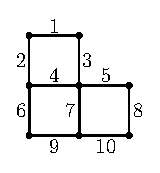
\includegraphics[scale=.9]{images/chap1/q10.eps}
\end{figure}

\item 12 ಬೆಂಕಿಕಡ್ಡಿಗಳಿಂದ ಚೌಕ ರಚಿಸಿದೆ. ಯಾವ ಎರಡು ಕಡ್ಡಿ ತೆಗೆದರೆ ಎರಡು ಚೌಕ ಮಾತ್ರ ಉಳಿಯುತ್ತವೆ ?
\vskip -.5cm
\begin{figure}[H]
\centering
\includegraphics[scale=.9]{images/chap1/q11.eps}
\end{figure}

\item 6 ಬೆಂಕಿಕಡ್ಡಿ ಜೋಡಿಸಿ 100 ಬರಿಸಿ.

\item ಈ ಗುಣಾಕಾರ ಗಮನಿಸಿ.
\begin{center}
\begin{tabular}{ccc}
$4\times 4$ & = & 16\\
$34\times 34$ & = & 1166\\
$334\times 334$ & = & 111666
\end{tabular}
\end{center}

ಹೀಗೆಯೇ ಮುಂದುವರಿಸಬಹುದು.

\item ಈ ಗುಣಾಕಾರ ಅಭ್ಯಸಿಸಿ.
\begin{align*}
& 1\times 2\times 3\times 4+1 = 5\times 5\\
& 2\times 3\times 4\times 5+1 = 11\times 11\\
& 3\times 4\times 5\times 6+1 = 19\times 19\\
& 4\times 5\times 6\times 7+1 = 29\times 29\\
& ...............................  \text{ ಹೀಗೆಯೇ ಮುಂದುವರಿಸಿ}
\end{align*}
\{ಎರಡು ಮತ್ತು ಮೂರನೆ ಅಂಕಿಗಳನ್ನು ಗುಣಿಸಿ, ಲಬ್ಧದಿಂದ 1 ಕಳೆದರೆ ವರ್ಗಸಂಖ್ಯೆ ಸಿಗುತ್ತದೆ.\}

\begin{tabbing}
ಉದಾ:\quad \= $2\times 3 =6$\\[2pt]
     \> $6-1=5$\\[3pt]
     \> $3\times 4=12$; \ $12-1=11$\\[2pt]
     \> $5\times 6=30$; \ $30-1=29$.
\end{tabbing}

\item 12345679 ಇದೊಂದು ವಿಶಿಷ್ಟ ಸಂಖ್ಯೆ. 1 ರಿಂದ 9 ರವರೆಗೆ ಕ್ರಮವಾಗಿ ಬರೆದಿದೆ, 8 ನ್ನು ಕೈ ಬಿಟ್ಟಿದೆ. ಈ ಸಂಖ್ಯೆಯ ಕೆಲವು ಗುಣಾಕಾರ ಪ್ರಕ್ರಿಯೆ ಗಮನಿಸಿ.
\begin{itemize}
\itemsep=4pt
\item[(a)] $12345679\times 8 = 98765432$

\item[(b)] $12345679\times 9 = 111 \ 111 \ 111$

ಹೀಗೆಯೇ 9 ರ ಮಗ್ಗಿ ಸಂಖ್ಯೆಗಳಿಂದ ಗುಣಿಸಿ ನೋಡಿ (18, 27...)

\item[(c)] $12345679\times 3 = 037 \ 037 \ 037$


$12345679 \times 6 = 074 \ 074 \ 074$


$12345679 \times 12 = 148 \ 148 \ 148$


78 ರವರೆಗೆ 3 ರ ಗುಣಕಗಳಿಂದ (9 ರ ಮಗ್ಗಿ ಸಂಖ್ಯೆ ಹೊರತುಪಡಿಸಿ) ಗುಣಿಸಿ ನೋಡಿ.
$$
12345679\times 78 = 962 \ 962 \ 962
$$ 
ಯಾವಾಗಲೂ 3 ಅಂಕಿಗಳ ಪುಂಜ ಮೂರು ಬಾರಿ ಬರುತ್ತದೆ.
\end{itemize}

\item ಈ ಚಿತ್ರದಲ್ಲಿರುವ ಆಕೃತಿಯಲ್ಲಿ ಎಷ್ಟು ಆಯತಗಳಿವೆ ?
\begin{figure}[!ht]
\centering
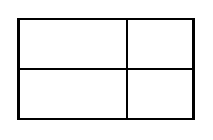
\includegraphics[scale=1.3]{images/chap1/q16.eps}
\end{figure}

\eject

\item ಈ ಆಕೃತಿಯಲ್ಲಿ 12 ವೃತ್ತಗಳಿವೆ. 1 ರಿಂದ 12 ವರೆಗಿನ ಸಂಖ್ಯೆಗಳನ್ನು ಪ್ರತಿ ವೃತ್ತದಲ್ಲಿಯೂ 1 ರಂತೆ ತುಂಬಿಸಿ. ಯಾವುದೇ ಸಾಲಿನ 4 ವೃತ್ತಗಳೊಳಗಿನ ಸಂಖ್ಯೆಗಳ ಮೊತ್ತ 26 ಬರಬೇಕು.
\begin{figure}[!ht]
\centering

\includegraphics[scale=.8]{images/chap1/q17.eps}
\end{figure}

\item ನಾಲ್ಕು ಚೌಕಾಕೃತಿಯ ಬಿಲ್ಲೆಗಳನ್ನು ಕತ್ತರಿಸಿ. (2 ಸೆಂ.ಮೀ. $\times$ 2 ಸೆಂ.ಮೀ.) ಇವುಗಳನ್ನು ಪರಸ್ಪರ ಲಗತ್ತಿಸಿರುವಂತೆ ಎಷ್ಟು ಬಗೆಗಳಲ್ಲಿ ಜೋಡಿಸಬಹುದು.

\item ನಾಲ್ಕು ಬಿಂದುಗಳು ಒಂದು ಚೌಕದ ಮೂಲೆಗಳಂತೆ ಇವೆ. ಇವುಗಳ ಮೂಲಕ ಹಾದು ಹೋಗುವಂತೆ 3 ಸರಳರೇಖೆಗಳನ್ನು ಎಳೆಯಬೇಕು. ಪೆನ್ಸಿಲ್‌ನ್ನು  ಕಾಗದದಿಂದ ಎತ್ತಬಾರದು, ಹಿಮ್ಮುಖ ಹೋಗುವಂತಿಲ್ಲ, ಹೇಗೆ? 
\begin{figure}[H]
\centering
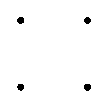
\includegraphics{images/chap1/q19.eps}
\end{figure}

\item ಅಲಿಕುಲದಲ ಮೂಲಂ ಮಾಲತೀಂ ಯಾತಮಷ್ಟೌ 

ನಿಖಿಲನವಮಭಾಗಾಶ್ಚಾಲಿನೀ ಭೃಗಮೇಕಂ ।

ನಿಶಿಪರಿಮಲ ಲುಬ್ಧಂ ಪದ್ಮ ಮಧ್ಯೇ ನಿರುದ್ಧಂ

ಪ್ರತಿರಣತಿ ರಣಂತಂ ಬ್ರೂಹಿ ಕಾಂತೇಽಳಿ ಸಂಖ್ಯಾಂ ।।

\hfill (ಭಾಸ್ಕರಾಚಾರ್ಯ (ಕ್ರಿ.ಶ. 522)ರ 'ಲೀಲಾವತೀ' ಗ್ರಂಥದಿಂದ)

\medskip

{\bf ಅರ್ಥ:} ಎಲೆ ಕಾಂತೆ! ಒಂದು ದುಂಬಿ (ಭೃಂಗ)ಗಳ ಸಮೂಹವಿತ್ತು. ಅದರ ಅರ್ಧ ಭಾಗದ ವರ್ಗ ಮೂಲದಷ್ಟು ದುಂಬಿಗಳು ಮಾಲತೀ ಪುಷ್ಪಗಳ ಕಡೆಗೆ ತೆರಳಿದುವು. ಒಂಭತ್ತನೇ ಭಾಗದ 8 ರಷ್ಟು ಹಾಗೇ ಹೋದುವು. ತಾವರೆ ಹೂವಿನೊಳಗೆ ಸಿಕ್ಕಿಕೊಂಡು ಒಂದು ದುಂಬಿ ಝೇಂಕರಿಸುತ್ತಿರಲು, ಇನ್ನೊಂದು ದುಂಬಿ ಆ ತಾವರೆಯ ಹೊರಗೆ ಸುತ್ತುತ್ತಿತ್ತು. ದುಂಬಿಗಳ ಒಟ್ಟು ಸಂಖ್ಯೆ ಎಷ್ಟು ಹೇಳು.

\eject

\item ವನಾಂತರಾಲೇ ಪ್ಲವಗಾಷ್ಟಭಾಗಃ ಸಂವರ್ಗಿತೋ ವಲ್ಗತಿ ಜಾತರಾಗ:

 ಫೂತ್ಕಾರ ನಾದ ಪ್ರತಿನಾದ ತುಷ್ಟಾ  ದೃಷ್ಟಾ ಗಿರೌ ದ್ವಾದಶತೇ ಕಿಯಂತಃ ।।

\hfill \{ಭಾಸ್ಕರಾಚಾರ್ಯರ `ಲೀಲಾವತಿ'ಯಿಂದ\}

{\bf ಅರ್ಥ:} ಒಂದು ಗುಂಪಿನಲ್ಲಿನ ಕೋತಿಗಳ $\frac{1}{8}$ ಭಾಗದ ವರ್ಗದಷ್ಟು ಕಾಡಿನಲ್ಲಿ ಕ್ರೀಡಿಸುತ್ತಿವೆ. 12 ಕೋತಿಗಳು ಕಿರಿಚಾಡುತ್ತಾ ಬೆಟ್ಟದ ಮೇಲೆ ಇವೆ. ಒಟ್ಟು ಕೋತಿಗಳೆಷ್ಟು?

\item ಒಬ್ಬ ಯುವಕ, ಒಬ್ಬಳು ಯುವತಿಯರ ಸಂವಾದ ಈ ರೀತಿ ಇದೆ.
\begin{description}
\item[ಯುವಕ:] ಎಲೆಲೆ ಬೆಡಗಿ, ಸುಂದರಿ ಚಲುವೆ ಆಗುವೆಯಾ ನೀನೆನ್ನ ಮದುವೆ?
\item[ಯುವತಿ:] ಅದಕೇನು ಕಷ್ಟ ಈಗಲೆ ಸಿದ್ಧ ಬಿಡಿಸು ನನ್ನೀಪದಿರ, ಮದುವೆಗೆ ನಾ ಬದ್ಧ.  [ಪದಿರು - ಒಗಟು, ಸಮಸ್ಯೆ]
\item[ಯುವಕ:] ಹೇಳು ಹೇಳು ಅದೇನು ಪದಿರು, ಕ್ಷಣದಲಿ ಬಿಡಿಸುವೆ ನೀನೋಡುತಿರು. 
\item[ಯುವತಿ:] ಇಲ್ಲಿವೆ ಸಸಿಗಳು ಎರಡು ಹತ್ತು ಮೇಲೈದು ಹನ್ನೆರಡು ಸಾಲುಗಳು ಪ್ರತಿಸಾಲಿಗೆ ಐದು ಸಸಿ ಬರುವಂತೆ ಹೊಂದಿಸುತಿಯೇನು? ಅದಾದರೆ ನಿನ್ನ ಮಡದಿಯಾಗುವೆನಾನು.
\item[ಯುವಕ:] ಸಾಧಿಸಿದ ಹೇಗೆ?
\end{description}

\item ಎಷ್ಟು $\frac{1}{4}$ “ಘನಗಳು 1" ಘನ ಮಾಡುತ್ತವೆ?

\item ರಾಜು ಒಂದು ಸ್ಟಾಂಪ್ ಹಾಳೆ ತಂದ. ಅದರಲ್ಲಿ 6 $\times$ 4 ಒಟ್ಟು 24 ಸ್ಟಾಂಪ್ ಇದ್ದುವು. ಪರಸ್ಪರ ಲಗತ್ತಾಗಿರುವ 3 ಸ್ಟಾಂಪ್‌ಗಳ 8 ಭಾಗ ಮಾಡಿದ. ಎರಡು ವಿಧಾನಗಳಲ್ಲಿ ಮಾಡಿತೋರಿಸಿದ. ಎರಡನ್ನು ಬರೆಯಿರಿ.

\item “1 $\times$ 2" ಆಯತ ರಚಿಸಿ. “1" ಚೌಕಗಳಾಗಿ ವಿಭಾಗಿಸಿ. ಕರ್ಣ ಎಳೆಯಿರಿ. 
\begin{figure}[H]
\centering

\includegraphics{images/chap1/q25a.eps}
\end{figure}

ಕರ್ಣ 2 ಮನೆಗಳ ಮೂಲಕ ಹಾದು ಹೋಗಿದೆ.


ಇದನ್ನೇ “2 $\times$ 3" ಆಯತದಲ್ಲಿ ಮಾಡಿ 
\begin{figure}[H]
\centering
\includegraphics{images/chap1/q25b.eps}
\end{figure}

ಕರ್ಣವು 4 ಮನೆಗಳ ಮೂಲಕ ಹಾದು ಹೋಗಿದೆ. 


“6 $\times$ 7" ಆಯತದಲ್ಲಿ ಎಷ್ಟು ಮನೆಗಳ ಮೂಲಕ ಹಾದು ಹೋಗುತ್ತದೆ? 

ಒಂದು ಸೂತ್ರ ರಚಿಸಬಹುದೆ? ಯತ್ನಿಸಿ.

\item ಪ್ರತಿಯೊಂದರಲ್ಲಿಯೂ 5 ಉಂಗುರಗಳಿರುವ 6 ಸರಪಳಿಗಳಿವೆ. ಇದನ್ನು ವೃತ್ತಾಕಾರದ ಸರಮಾಡಿಸಬೇಕು. 1 ಉಂಗುರ ಕತ್ತರಿಸಲು 2 ರೂ, 1 ಬೆಸುಗೆಗೆ 3 ರೂ ಆದರೆ, ಸರ ಮಾಡಿಸಲು ಬೇಕಾಗುವ ಅತಿ ಕಡಿಮೆ ಹಣ ಎಷ್ಟು?

\item 3 ಅಥವಾ ಅದರ ಯಾವುದೇ ಗುಣಕವನ್ನು ತೆಗೆದುಕೊಳ್ಳಿ. ಅಂಕಿಗಳ ಘನ ಮಾಡಿ ಕೂಡಿ. ಬಂದ ಉತ್ತರದಲ್ಲಿಯೂ ಅಂಕಿಗಳ ಘನ ಮಾಡಿ ಮೊತ್ತ ಪಡೆಯಿರಿ. ಮತ್ತೆ ಘನ ಮಾಡುವ ಮತ್ತು ಅಂಕಿಗಳ ಮೊತ್ತ ಮಾಡುವ ಪ್ರಕ್ರಿಯೆ ಮುಂದುವರಿಸಿ. ಯಾವಾಗಲೂ ಅಂತಿಮ ಉತ್ತರ 153

{\bf ಉದಾ:} 3
\begin{align*}
 3^{3} = 27&; 2^{3} + 7^{3} = 8 + 343 = 351\\
3^{3} + 5^{3} + 1^{3} & = 27 + 125 + 1 = 153
\end{align*}

ಯಾವುದೇ 3ರ ಗುಣಕ (ಎಷ್ಟೇ ದೊಡ್ಡ ಸಂಖ್ಯೆಯಾದರೂ) ಅಂತಿಮ ಉತ್ತರ 153

\item ಒಂದು ವಿಶಿಷ್ಟ ಸಂಖ್ಯಾಮಾಲೆ
\begin{figure}[H]
\centering
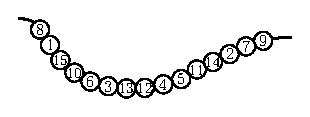
\includegraphics{images/chap1/q28.eps}
\end{figure}

1 ರಿಂದ 15 ವರೆಗಿನ ಸಂಖ್ಯೆಗಳನ್ನು ಒಮ್ಮೆ ಮಾತ್ರ ಬಳಸಿದೆ. ಯಾವುದೇ 2 ಅನುಕ್ರಮ ಸಂಖ್ಯೆಗಳ ಮೊತ್ತ ವರ್ಗ ಸಂಖ್ಯೆ

{\bf ಉದಾ:}
\begin{tabular}[t]{ll}
$8 + 1 = 9$ & $12 + 4 = 16$\\
$1 + 15 = 16$ & $4 + 5 = 9$
\end{tabular}

\hfill (ಜಪಾನಿ ಗಣಿತಜ್ಞ ನೊಬುಯುಕಿ ಯೋಷಿಗಹಾರ ಅವರ ರಚನೆ).

\item ಸಂಖ್ಯೆಗಳನ್ನು ಸಮ (even) ಮತ್ತು ಬೆಸ (odd) ಎಂದು ವಿಭಾಗಿಸಬಹುದು ಬೆಸ\break ಸಂಖ್ಯೆಗಳು $1, 3, 5, 7, \ldots$ ಇವುಗಳ ಮೊತ್ತ ನೋಡೋಣ

{\fontsize{11pt}{13pt}\selectfont
\begin{tabular}{lll}
$1 + 3 = 4$ &(ಎರಡು ಕ್ರಮಾಗತ ಬೆಸ ಸಂಖ್ಯೆಗಳು) & = $2^{2}$\\
$1 + 3 + 5 = 9$ &(3 ಸಂಖ್ಯೆಗಳು) & = $3^{2}$\\
$1 + 3 + 5 + 7 = 16$ &(4 ಸಂಖ್ಯೆಗಳು) & = $4^{2}$\\
ಹೀಗೆಯೇ & n ಸಂಖ್ಯೆಗಳು & = $n^{2}$
\end{tabular}}\relax

ಇದೇರೀತಿ ಸಮ ಸಂಖ್ಯೆಗಳ ಮೊತ್ತದ ಸೂತ್ರ ನೋಡೋಣ $2, 4, 6, 8, \ldots$ ಸಮ ಸಂಖ್ಯೆಗಳು

{\fontsize{11pt}{13pt}\selectfont
\begin{tabular}{lll}
$2 + 4= 6$ & ಎರಡು ಸಂಖ್ಯೆಗಳು & $2(2 + 1) = 2 \times 3 = 6$\\
$2 + 4 + 6 = 12$ & ಮೂರು ಸಂಖ್ಯೆಗಳು & $3(3 + 1) = 3 \times 4 = 12$\\
$2 + 4 + 6 + 8 = 20$ &ನಾಲ್ಕು ಸಂಖ್ಯೆಗಳು & $4(4 + 1) = 4 \times 5 = 20$\\
$n$ ಸಂಖ್ಯೆಗಳಿದ್ದರೆ & $n(n + 1)$ ಸೂತ್ರ &
\end{tabular}}\relax

\item 2201$^{3}$ = 10662526601

ಒಂದು ಸಂಖ್ಯೆಯ ಘನ ಮಾಲಾ ಸಂಖ್ಯೆ. ಸದ್ಯದಲ್ಲಿ ಲಭ್ಯರಿರುವುದು ಇದೊಂದೇ.
\end{enumerate}

\smallskip

\begin{center}
\rule{5cm}{1pt}\\[2pt]
{\Large\bfseries ಉತ್ತರಗಳು}\\[-0.1cm]
\rule{5cm}{1pt}
\end{center}


\begin{enumerate}
\itemsep=5pt

\item $1 + 1 + 11 + 11 = 24$

\smallskip
\item $(1, 8), (2, 7), (3, 6), (4, 5)$

\smallskip
\item 
\begin{tabbing}
~~~$1$ \= = \= $2 + 2 - 2 - \dfrac{2}{2}$\\[0.2cm]
~~~$2$ \> = \> $2 + 2 + 2 - 2 - 2$\\[0.2cm]
~~~$3$\> = \> $2 + 2 - 2 + \dfrac{2}{2}$\\[0.2cm]
~~~$4$ \> = \> $2 \times 2 \times 2 - 2 - 2$\\[0.2cm]
~~~$5$ \> = \> $2 + 2 + 2 - \dfrac{2}{2}$\\[0.2cm]
~~~$6$ \> = \> $2 + 2 + 2 + 2 - 2$\\[0.2cm]
~~~$7$ \> = \> $(22 \div 2) - 2 - 2$\\[0.2cm]
~~~$8$ \> = \> $(2 \times 2 \times 2 \times 2) \div 2$\\[0.2cm]
~~~$9$ \> = \> $2 \times 2 \times 2 + \dfrac{2}{2}$\\[0.2cm]
$10$~ \> = \> $2 + 2 + 2 + 2 + 2$
\end{tabbing}

\smallskip
\item $6 + 6 +\left\{\dfrac{6}{6} + \dfrac{6}{6}\right\}$

\smallskip
\item $22 + 2 = 24$

\item 
\begin{tabbing}
$6 \times 6 - 6$ \qquad\=  = \= $30$\\
$5 \times 5 + 5$ \qquad\>  = \> $30$\\
$33 - 3$ \qquad\>  = \> $30$\\
$4! + 4 + \sqrt{4}$ \> = \> $30$\\
$10 + 10 + 10$ \qquad\> = \> $30$
\end{tabbing}

\item 
\begin{itemize}
\item[(a)] VI $+$ IV = X \{XIರ 1 ನ್ನು $-$ ಮೇಲೆ ಹಾಕಿದೆ\}
\item[(b)] V $-$ IV = $\sqrt{1}$ \{VIIರ 1 ನ್ನು ಮೇಲೆ ಅಡ್ಡ ಹಾಕಿದೆ.\}
\end{itemize}

\smallskip
\item $\dfrac{11}{VI} = \dfrac{2}{6} = \dfrac{1}{3}$ \{VII ರ 1 ನ್ನು ಅಂಶದಲ್ಲಿ ಬರೆದಿದೆ.\}

\smallskip
\item 9 ಬೆಂಕಿ ಕಡ್ಡಿಗಳಿಂದ 4 ಸಮಬಾಹು ತ್ರಿಭುಜ ರಚಿಸಬಹುದು 
\begin{figure}[H]
\centering

\includegraphics{images/chap1/ans9.eps}
\end{figure}

\eject

\item 6 ಮತ್ತು 9 ತೆಗೆಯಬೇಕು. 
\begin{figure}[H]
\centering
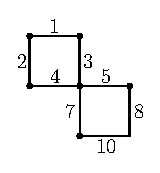
\includegraphics{images/chap1/ans10.eps}
\end{figure}

\item 
~

\begin{minipage}[c]{5cm}
\begin{figure}[H]
\centering
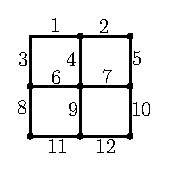
\includegraphics{images/chap1/ans11.eps}
\end{figure}
\end{minipage}
\begin{minipage}[c]{5cm}
\begin{tabular}{cc}
$(4,6)$ & \multirow{4}{3cm}{ಯಾವ 2 ಕಡ್ಡಿ ತೆಗೆದರೂ 2 ಚೌಕ ಮಾತ್ರ ಉಳಿಯುತ್ತದೆ.}\\
$(4,7)$ & \\
$(6,9)$ &\\
$(7,9)$ & 
\end{tabular}
\end{minipage}


\medskip
\item 
~

\begin{tabular}[t]{cc}

\includegraphics{images/chap1/ans12.eps} & \raisebox{.7cm}{$= 100 = \left\{\overline{X} = 10000\right\}$}
\end{tabular}

\item ಉತ್ತರದ ಅಗತ್ಯವಿಲ್ಲ 

\item ಉತ್ತರದ ಅಗತ್ಯವಿಲ್ಲ 

\item ಉತ್ತರದ ಅಗತ್ಯವಿಲ್ಲ 

\item 9 ಆಯತಗಳು 


\item ಪ್ರತಿ ಸಾಲಿನ 4 ಸಂಖ್ಯೆಗಳ ಮೊತ್ತ  26
\begin{figure}[H]
\centering
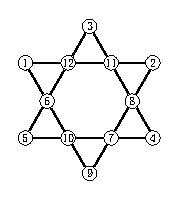
\includegraphics{images/chap1/ans17.eps}
\end{figure}

\eject

\item 5 ವಿಧಗಳಲ್ಲಿ ಜೋಡಿಸಬಹುದು.
\begin{figure}[H]
\centering
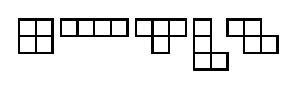
\includegraphics{images/chap1/ans18.eps}
\end{figure}



\item 
~

\begin{figure}[H]
\centering
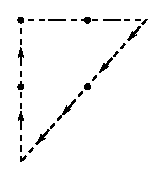
\includegraphics{images/chap1/ans19.eps}
\end{figure}

\item ಇದು ವರ್ಗ ಸಮೀಕರಣದ ಸಮಸ್ಯೆ ದುಂಬಿಗಳ ಸಂಖ್ಯೆ  $x$ ಇರಲಿ ಅರ್ಧಭಾಗದ ವರ್ಗಮೂಲ $\sqrt{\dfrac{x}{2}}$ ಅಥವಾ $\dfrac{\sqrt{x}}{\sqrt{2}}$ ಒಂಭತ್ತನೆ ಭಾಗದ 8ರಷ್ಟು $\dfrac{8x}{9}$ $\dfrac{\sqrt{x}}{\sqrt{2}} + \dfrac{8x}{9} + 1 + 1 = x$ ಸಮೀಕರಣ ಸಿದ್ಧಿಸುತ್ತದೆ. 
\begin{align*}
\text{ಬಿಡಿಸಿದಾಗ}\quad \dfrac{\sqrt{x}}{\sqrt{2}} & = x - \dfrac{8x}{9} - 2\\
\dfrac{\sqrt{x}}{\sqrt{2}} & = \dfrac{x}{9} - 2\\
\text{ವರ್ಗಣೆಯಿಂದ}\quad \dfrac{x}{2} & = \left(\dfrac{x}{9} - 2\right)^{2}\\
\dfrac{x}{2} & = \dfrac{x^{2}}{81} - \dfrac{4x}{9} + 4
\end{align*}
162 ರಿಂದ ಗುಣಿಸಿ 
\begin{align*}
& 81x = 22 - 72x + 648\\
& 2x^{2} - 153x + 648 = 0\\
& (2x - 9) (x - 72) = 0\\
& x = 72 \quad\text{ಅಥವಾ}\quad \dfrac{9}{2}\\
& x = 72 \quad\text{ಸರಿಯಾದ ಉತ್ತರ}\\
& 72\quad\text{ ದುಂಬಿಗಳು}
\end{align*}

\item ಕೋತಿಗಳ ಸಂಖ್ಯೆ  $x$ ಇರಲಿ 

\begin{tabular}{l|l}
$\left(\dfrac{x}{8}\right)^{2} + 12 = x$ & $x^{2} - 64x + 768 = 0$\\[6pt]
$\dfrac{x^{2}}{64} + 12 = x$ & $(x - 16) (x - 48) = 0$\\[6pt]
$x^{2} + 768 = 64x$ & $x = 16$\quad ಅಥವಾ 48\\[6pt]
& $\therefore$ ಕೋತಿಗಳ ಸಂಖ್ಯೆ 16 ಅಥವಾ 48
\end{tabular}

\smallskip
\item 
~

\noindent
\begin{minipage}[c]{4cm}
\begin{figure}[H]
\centering
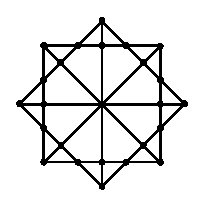
\includegraphics[scale=.85]{images/chap1/ans22.eps}
\end{figure}
\end{minipage}
\begin{minipage}[c]{5cm}
\begin{tabular}{lr}
2 ಚೌಕಗಳ ಬಾಹುಗಳು & 8\\
2 ಚೌಕಗಳ ಕರ್ಣಗಳು & 4\\
\hline
ಒಟ್ಟು ಸಾಲುಗಳು & 12\\
\hline
ಪ್ರತಿಯೊಂದರಲ್ಲೂ 5 ಸಸಿಗಳಿವೆ. &
\end{tabular}
\end{minipage}




\item 64 ಘನಗಳು 

\item 
\begin{tabular}[c]{c}

\includegraphics{images/chap1/ans24a.eps}\quad \raisebox{.3cm}{ಅಥವಾ} \quad 
\includegraphics{images/chap1/ans24b.eps}
\end{tabular}

\item “6 $\times$ 7" ಆಯತದಲ್ಲಿ ಕರ್ಣವು 12 ಮನೆಗಳ ಮೂಲಕ ಹಾದು ಹೋಗುತ್ತದೆ.

ಸೂತ್ರ ($l + b - 1$) ಕತ್ತರಿಸುವ ಚೌಕಗಳ ಸಂಖ್ಯೆ 

\item 1 ಸರಪಳಿಯ 5 ಉಂಗುರ ಕತ್ತರಿಸಿ . 5ನ್ನು ಕತ್ತರಿಸಲು 10ರೂ ಉಳಿದ 5 ಸರಪಳಿಗಳ ತುದಿಗಳನ್ನು ಕತ್ತರಿಸಿದ ಉಂಗುರ ಹಾಕಿ ಬೆಸೆಸಿ. 5 ಬೆಸಿಗೆಗೆ 15ರೂ 

ಅತಿಕಡಿಮೆ ಹಣ 15 $+$ 10 = 25ರೂ 

\item ಉತ್ತರ ಅಗತ್ಯವಿಲ್ಲ 

\item ಉತ್ತರ ಅಗತ್ಯವಿಲ್ಲ 

\item ಉತ್ತರ ಅಗತ್ಯವಿಲ್ಲ 

\item ಉತ್ತರ ಅಗತ್ಯವಿಲ್ಲ 
\end{enumerate}
